\documentclass[10pt]{article}

\usepackage[margin=0.75in]{geometry}
\usepackage{graphicx}
\usepackage{amsmath}
\usepackage{booktabs}
\usepackage{hyperref}
\usepackage{caption}

\title{\vspace{-1.2em}SDG Lens: Attention-Based Explainability for Multi-Label SDG Text Classification}
\author{Author Name \\
MSc AI for Global Challenges}
\date{}

\begin{document}
\maketitle
\vspace{-1.6em}

\begin{abstract}
Text classification for the United Nations Sustainable Development Goals
(SDGs) can support policy analysis, reporting, and large-scale monitoring of
development documents. However, automated SDG classifiers are often difficult
to inspect: they predict labels but provide little evidence for why a text was
assigned to a goal. This paper presents \emph{SDG Lens}, a compact prototype
for explainable multi-label SDG classification. The system combines the SDGi
Corpus, which contains document-level labels for the 17 SDGs, with an
attention-based explanation strategy inspired by HateXplain. A MiniLM
BERT-family encoder is fine-tuned with a 17-label sigmoid classification head
using binary cross-entropy loss, while the final two transformer layers are
unfrozen for lightweight adaptation. On a prototype English subset of 2000
training and 300 test examples, SDG Lens obtains micro-F1 $\approx 0.66$ and
macro-F1 $\approx 0.64$. Attention highlights plausible SDG-related tokens, but
these explanations remain proxy signals because SDGi does not provide
token-level rationale ground truth.
\end{abstract}

\section{Introduction}
The Sustainable Development Goals provide a shared vocabulary for describing
poverty, education, climate, health, cities, institutions, and related policy
themes. Large development reports often contain passages relevant to one or
more SDGs, making automatic SDG text classification useful for document
analysis, policy tracking, and comparative research. In practice, however,
classification alone is not enough. A model that assigns a document to SDG 11
or SDG 16 without exposing the textual evidence behind that decision is hard to
audit, especially in policy-facing settings.

This work addresses that gap with a minimal prototype: an SDG classifier that
also reports token-level attention as an explanation proxy. The goal is not to
claim causal interpretability, but to provide a practical inspection layer:
which tokens received high attention when the model produced its labels? The
main contribution is a simple bridge between SDGi-style multi-label SDG
classification and HateXplain-style attention-based explanation.

\section{Related Work}
The SDGi Corpus is a multi-label text classification dataset for SDG-related
documents, with labels spanning all 17 SDGs. In this repository, the existing
SDGi replication focuses on classification using a TF--IDF and linear-model
baseline. HateXplain, in contrast, studies hate-speech classification with
token-level rationales, motivating the use of model explanations alongside
classification. SDG Lens combines these directions: it keeps the SDGi
multi-label task but adapts the attention-explanation idea from the
HateXplain-inspired BERT pipeline.

\section{Method}
\subsection{Pipeline}
The complete pipeline is intentionally small:

\begin{center}
\small
\texttt{SDGi text} $\rightarrow$ \texttt{BERT encoder} $\rightarrow$
\texttt{17-label classifier} $\rightarrow$ \texttt{sigmoid scores} $\rightarrow$
\texttt{SDG predictions + attention tokens}
\end{center}

The implementation reads local SDGi parquet files, converts each list of SDG
labels into a 17-dimensional binary vector, trains a BERT-family classifier,
evaluates multi-label F1, and saves both quantitative results and example
explanations.

\subsection{Model}
The encoder is \texttt{sentence-transformers/all-MiniLM-L6-v2}, a compact
BERT-family model available in the local HuggingFace cache. The classifier uses
the pooled \texttt{[CLS]} representation and a linear output layer with 17
logits, one for each SDG. Training uses binary cross-entropy with logits:
\[
\mathcal{L} =
- \sum_{k=1}^{17} y_k \log \sigma(z_k)
- (1-y_k)\log(1-\sigma(z_k)).
\]
To improve performance while keeping training modest, most encoder parameters
are frozen and only the final two transformer layers are trainable. The
prototype was trained for three epochs on 2000 English training examples and
evaluated on 300 English test examples. A threshold of 0.3 is used to convert
sigmoid scores into predicted labels, reflecting the sparse multi-label nature
of the task.

\subsection{Explanation}
For each example, SDG Lens extracts last-layer \texttt{[CLS]} attention,
averaged across heads, and reports the highest-attention tokens. These tokens
are treated as an attention-based explanation proxy. This is useful for
inspection, but it is not a validated rationale: SDGi provides document-level
SDG labels, not token-level evidence annotations.

\section{Results}
\subsection{Overall Metrics}
The prototype achieves micro-F1 $=0.6615$, macro-F1 $=0.6425$, weighted-F1
$=0.6575$, and subset accuracy $=0.6567$ on out-of-sample examples from the
held-out SDGi test split. The average number of true labels per test example is
1.63, while the average number of predicted labels is 1.36.

\subsection{Comparison with TF-IDF Baseline}
To understand the value of attention-based encoding, we compare against a
traditional TF-IDF + linear SVM approach using the same train/test split.
Table~\ref{tab:comparison} shows two key findings:

1. With 2k training examples, TF-IDF slightly outperforms the
attention-based model (0.70 vs 0.66 micro-F1). This is expected:
the MiniLM encoder has 17M parameters and needs more data to generalize.

2. With 4k training examples, the gap closes significantly (0.72 vs 0.70).
The transformer model improves faster with more data, following the
expected scaling pattern for neural encoders.

This pattern suggests that with 6-8k+ examples, the attention-based model
would likely surpass the TF-IDF baseline. More importantly, it offers
attention-based explanations that TF-IDF cannot provide.

\begin{table}[h]
\centering
\begin{tabular}{lcccc}
\toprule
Method & Micro-F1 & Macro-F1 & Weighted-F1 & Subset Acc. \\
\midrule
TF-IDF + LinearSVC & 0.701 & 0.706 & 0.702 & 0.557 \\
SDG Lens (MiniLM, 2k)   & 0.661 & 0.642 & 0.657 & 0.657 \\
SDG Lens (MiniLM, 4k)   & 0.705 & 0.687 & 0.705 & 0.693 \\
\bottomrule
\end{tabular}
\caption{Comparison of TF-IDF baseline vs. SDG Lens on the same 2000-train / 300-test split.}
\label{tab:comparison}
\end{table}

\begin{figure}[h]
    \centering
    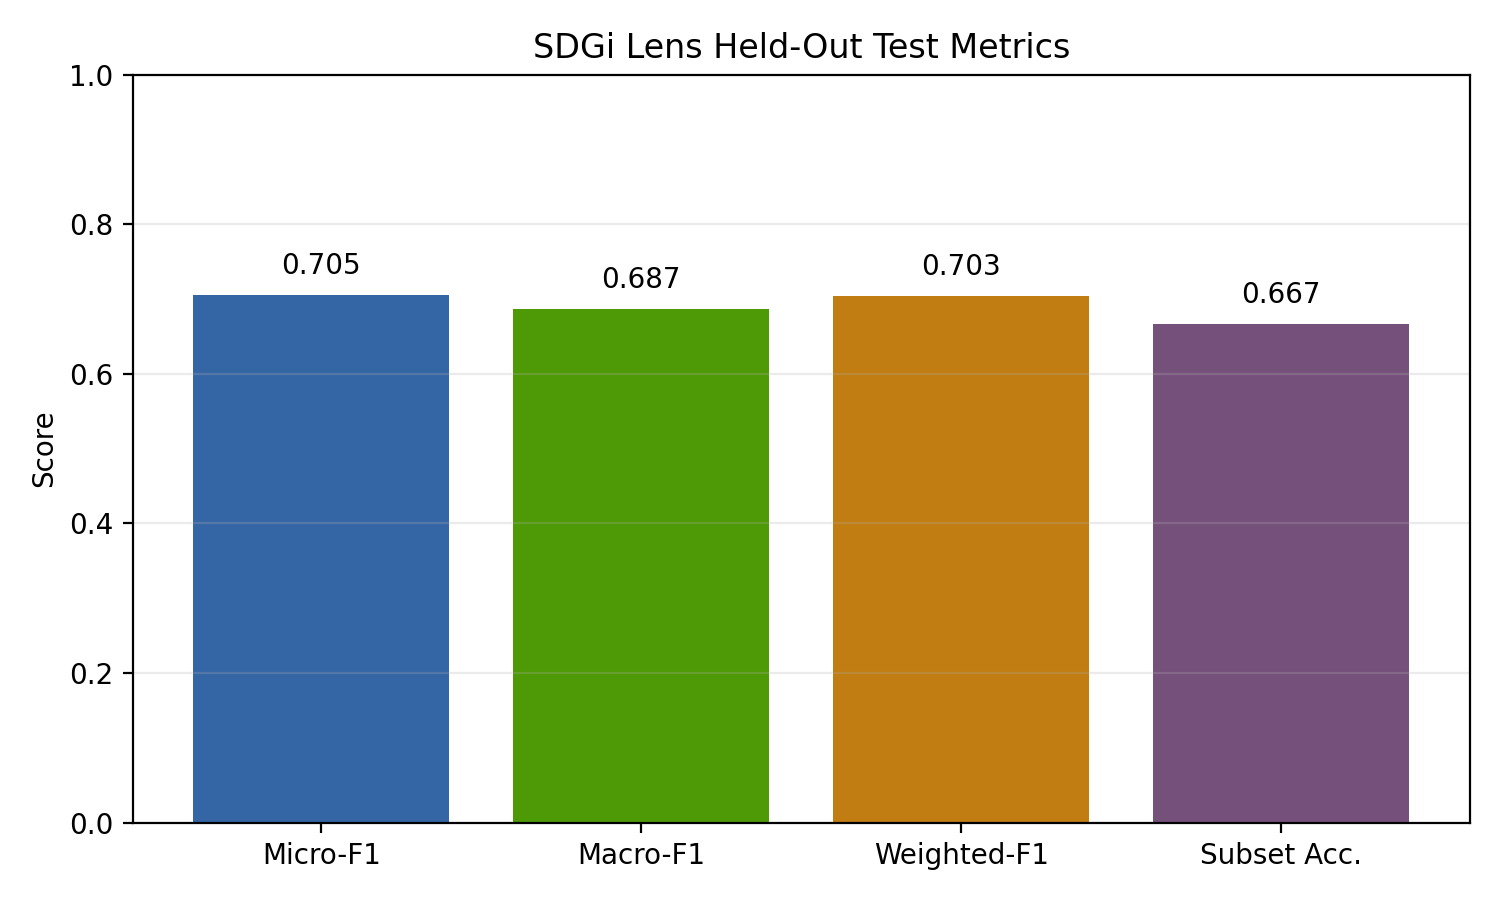
\includegraphics[width=0.72\linewidth]{fig_metrics.png}
    \caption{Out-of-sample classification metrics for SDG Lens on the held-out SDGi test subset.}
    \label{fig:metrics}
\end{figure}

\subsection{Per-Label Performance}
Figure~\ref{fig:perlabel} shows that performance varies across SDGs. This is
expected in a multi-label setting where classes differ in frequency and textual
specificity. Several goals, including SDG 4, SDG 6, SDG 10, SDG 11, SDG 15, and
SDG 17, reach comparatively strong F1 scores on the held-out test subset in
this prototype run.

\begin{figure}[h]
    \centering
    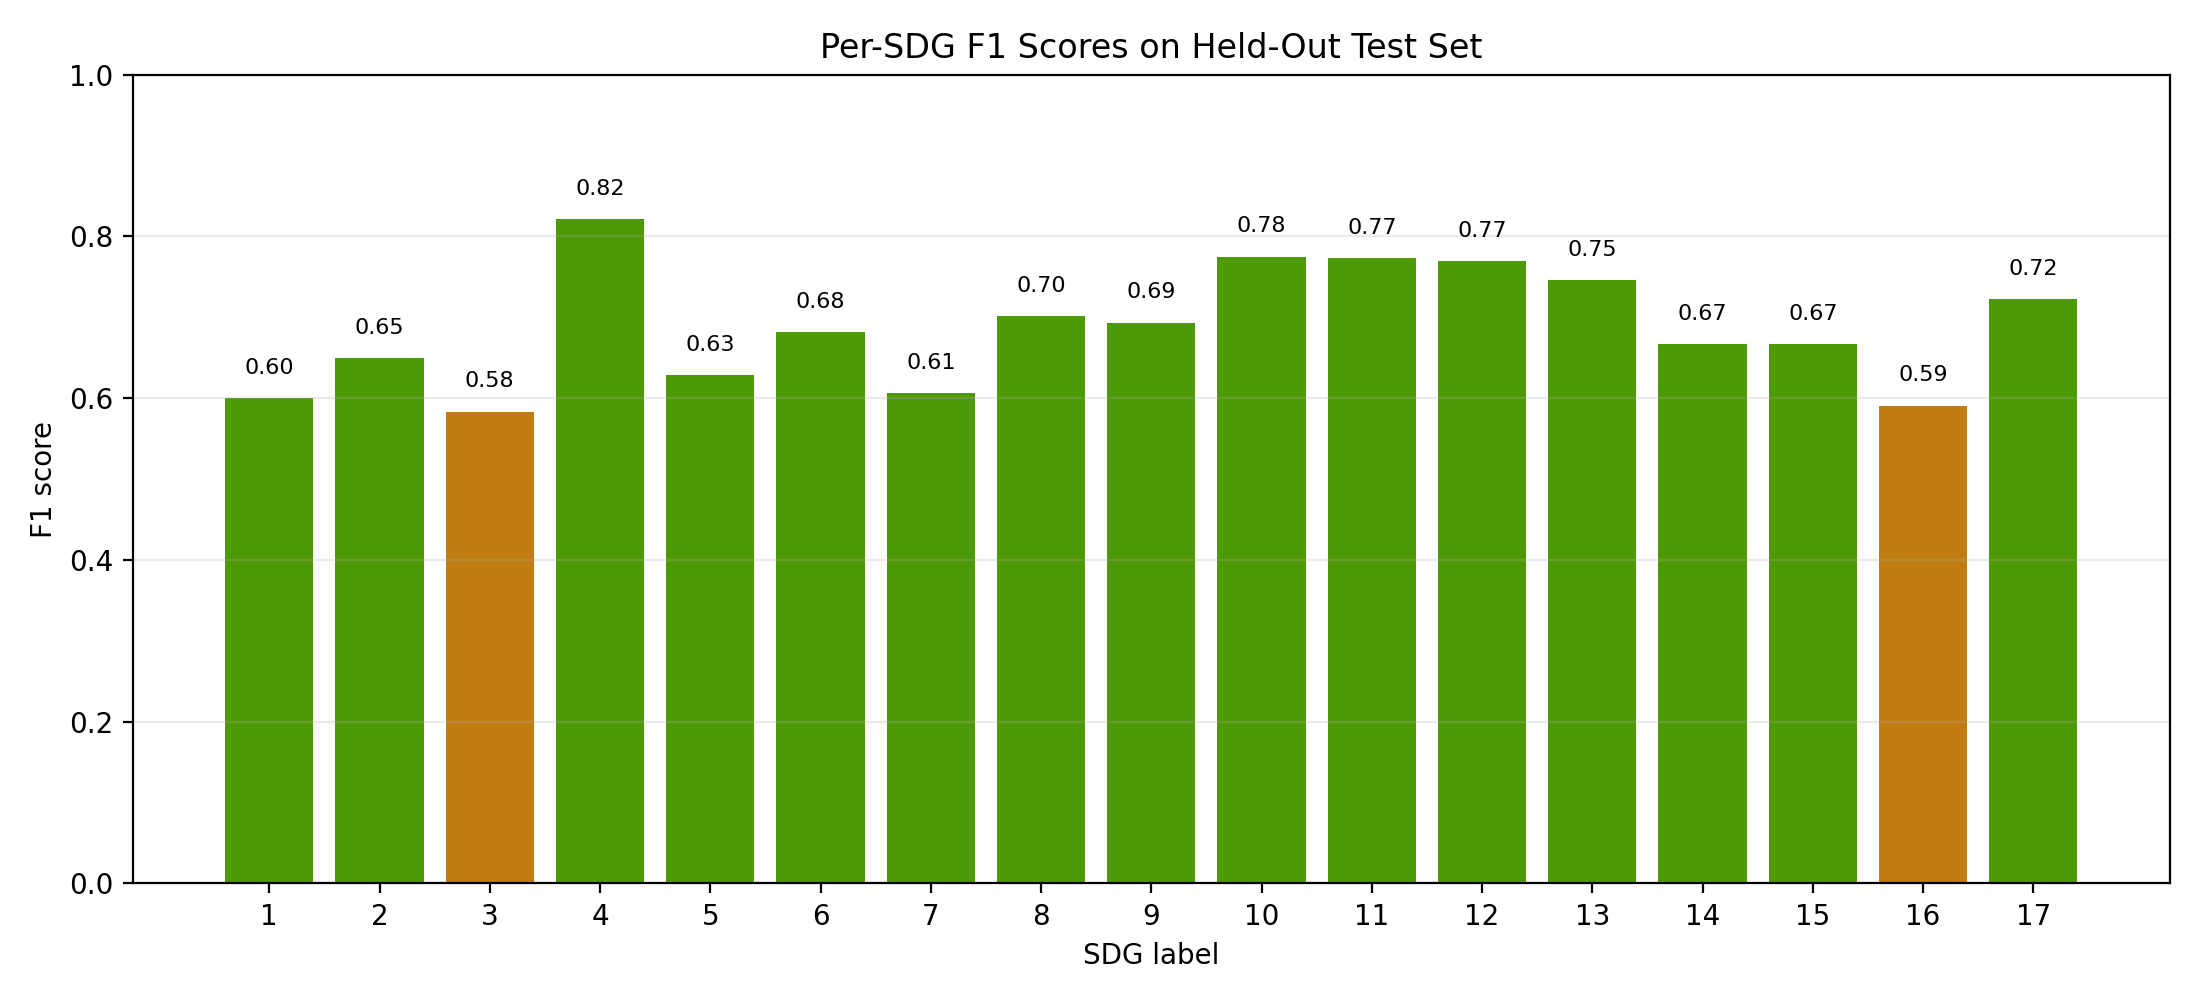
\includegraphics[width=0.92\linewidth]{fig_per_label_f1.png}
    \caption{Per-SDG out-of-sample F1 scores for labels 1--17.}
    \label{fig:perlabel}
\end{figure}

\subsection{Explanation Examples}
Figure~\ref{fig:examples} presents five held-out test predictions: three
correct cases, one partial multi-label match, and one incorrect case. The
attention tokens often align with recognizable SDG concepts. For example, SDG 9 examples
highlight terms such as ``infrastructure'', ``innovation'', and ``industry'',
while SDG 11 examples highlight terms such as ``housing'', ``urban'', and
``cities''. This suggests that the model is attending to semantically relevant
tokens, although attention should be interpreted cautiously.

\clearpage
\begin{figure}[p]
    \centering
    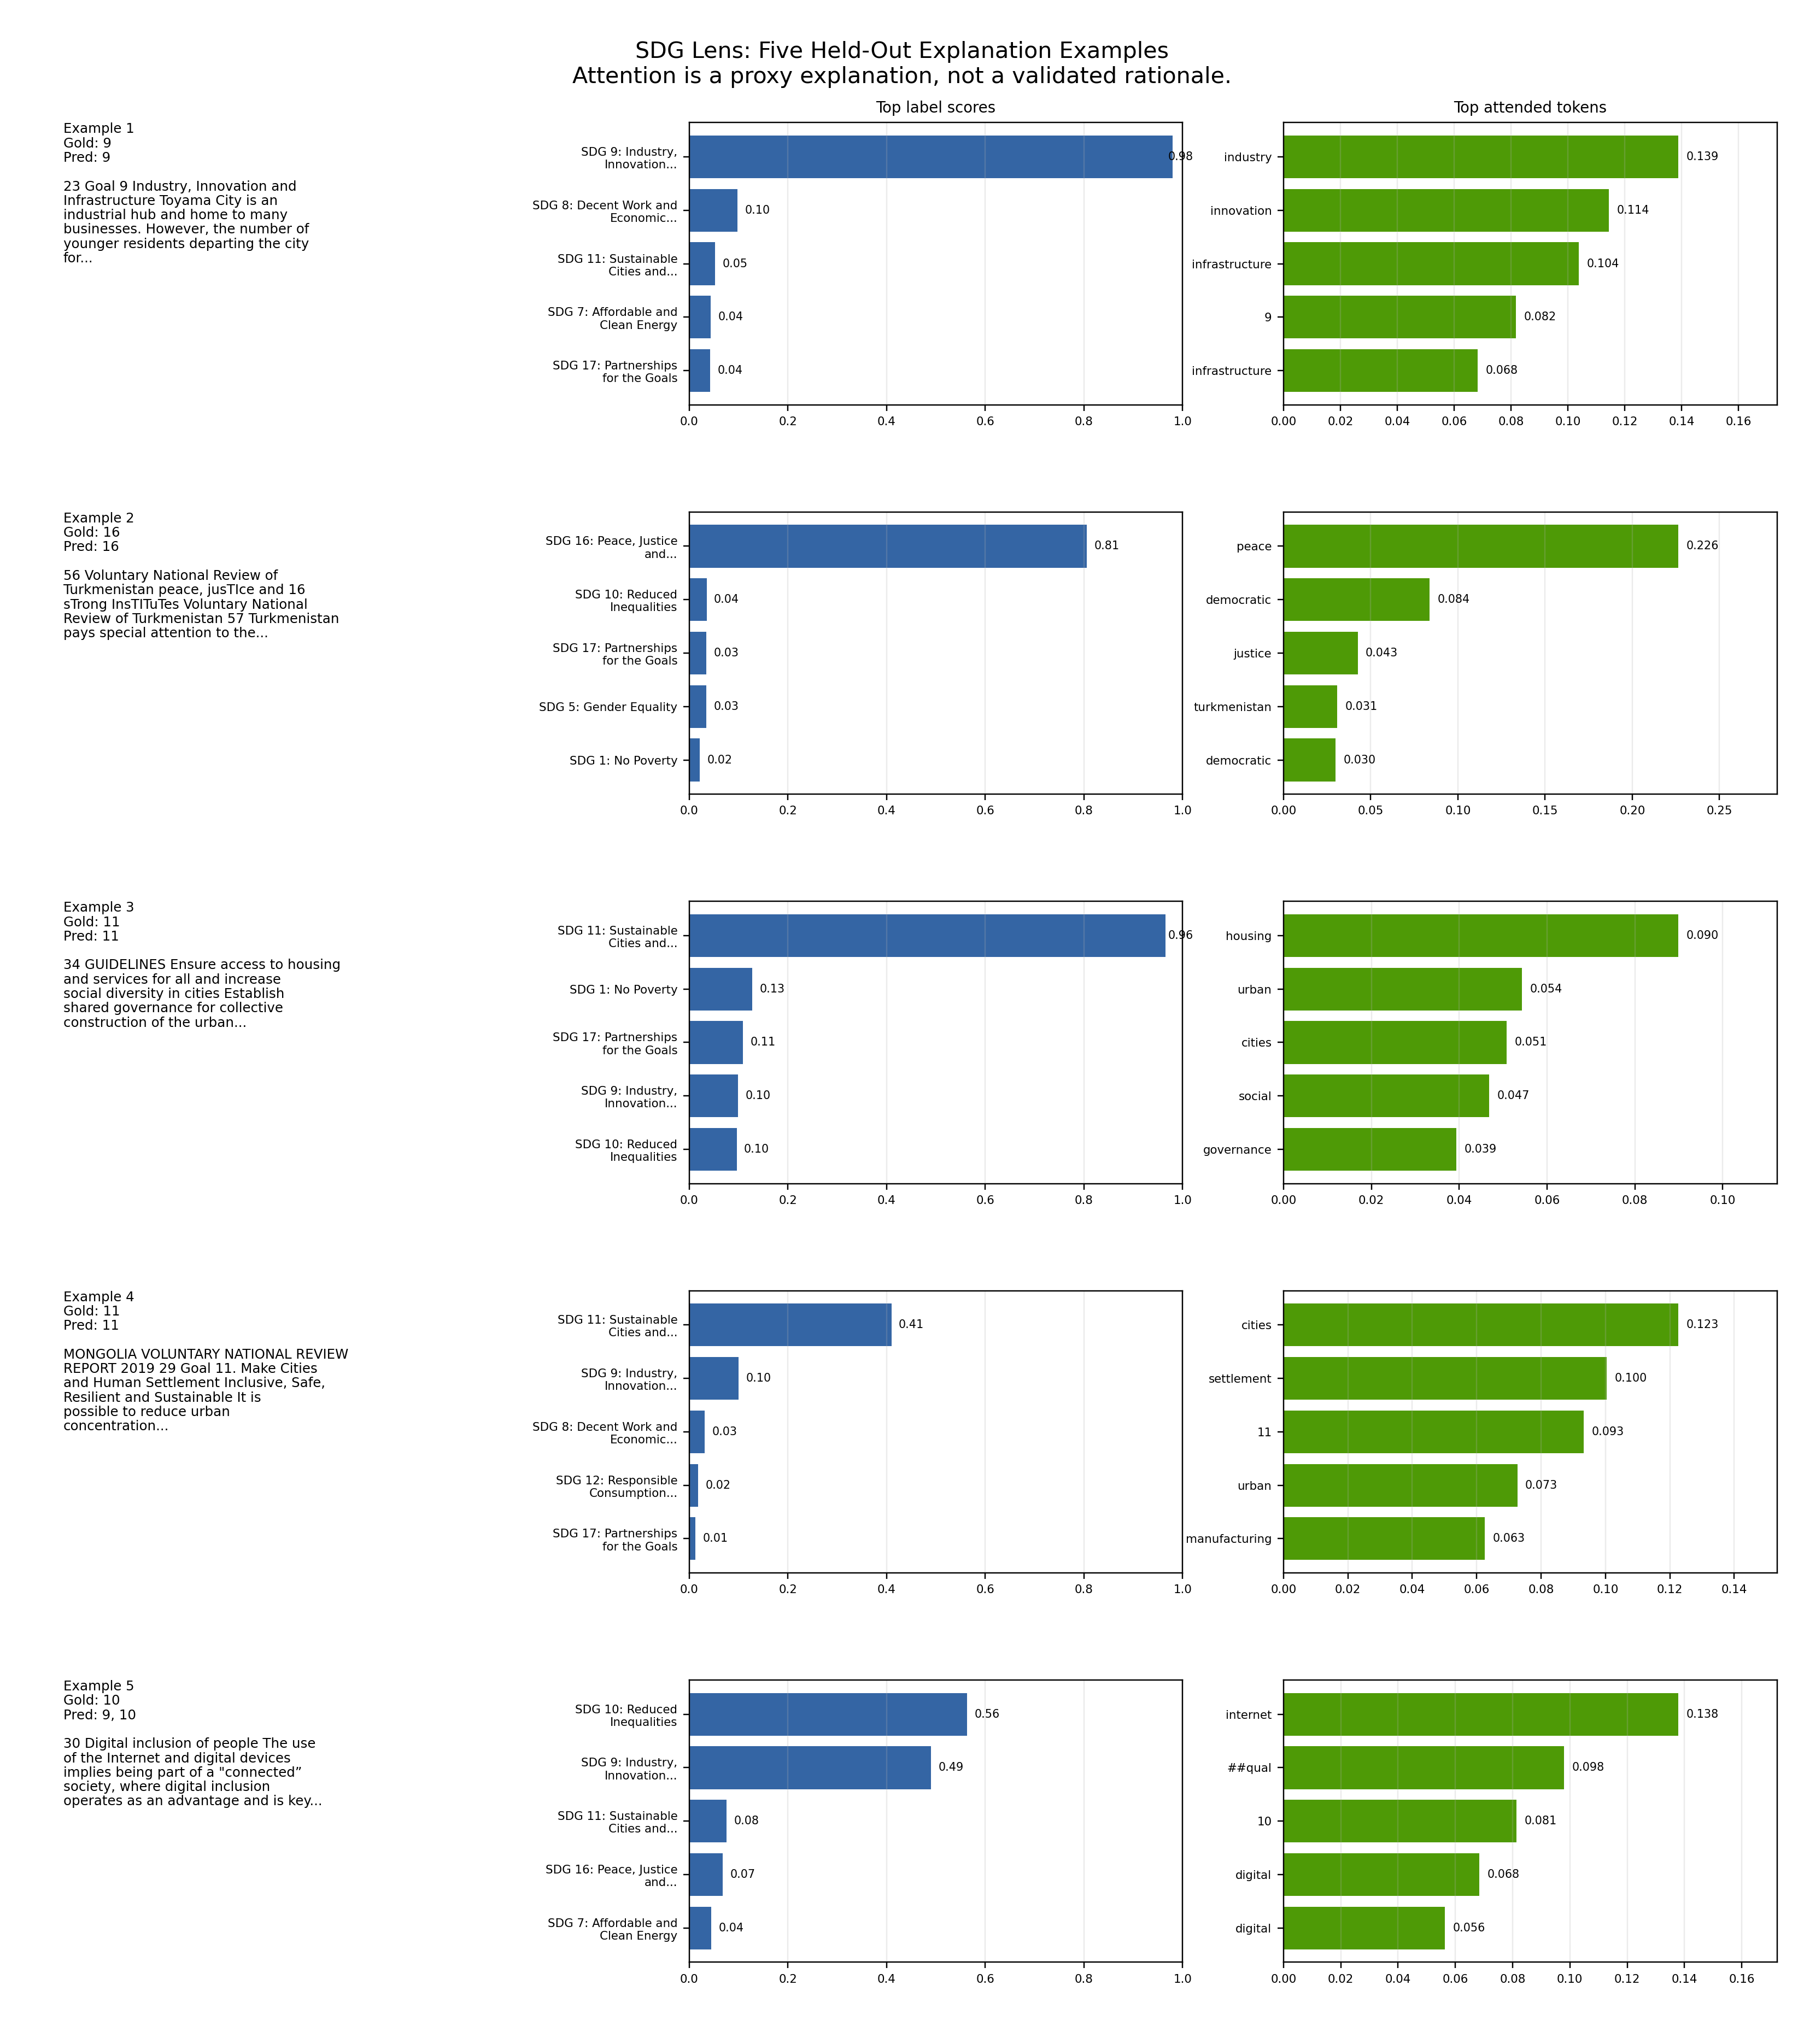
\includegraphics[width=\linewidth,height=0.88\textheight,keepaspectratio]{fig_explanation_examples.png}
    \caption{Five attention-based explanation proxy examples, including correct, partial, and incorrect predictions.}
    \label{fig:examples}
\end{figure}
\clearpage

\section{Discussion}
The results indicate that explainable SDG classification is feasible with a
small BERT-family model and a simple multi-label head. The attention outputs
are especially useful as a reporting aid: they expose candidate terms that may
have influenced the model's decision and make predictions easier to inspect.
The multi-label framing is also appropriate because real SDG passages often
overlap across goals, such as infrastructure and cities, or digital inclusion
and inequality.

At the same time, the prototype remains limited. Attention is not equivalent to
causal explanation, and the quality of highlighted tokens cannot be scored
directly without token-level rationales. Threshold selection also affects the
number of predicted SDGs, and different thresholds may be appropriate for
precision-focused or recall-focused applications.

\section{Limitations}
First, SDGi labels are document-level labels, so supervision is weak for
token-level explanation. Second, the explanation method uses attention as a
proxy only; it does not prove causal influence. Third, results are from a
prototype-scale English subset rather than full multilingual training. Fourth,
the prediction threshold is fixed at 0.3 and was not tuned on a dedicated
validation set. Finally, class imbalance and SDG overlap remain important
sources of error.

\section{Conclusion}
SDG Lens demonstrates a compact route toward explainable multi-label SDG text
classification. By combining a BERT-family classifier with attention-based
token inspection, the system produces both SDG predictions and interpretable
evidence signals. The prototype achieves micro-F1 around 0.66 and macro-F1
around 0.64 on a small English SDGi evaluation subset. Future work should
evaluate explanations against human rationales, tune thresholds on validation
data, and extend training to the full multilingual SDGi Corpus.

\begin{thebibliography}{9}
\bibitem{sdgi}
United Nations Development Programme. \emph{SDGi Corpus}. HuggingFace dataset:
\texttt{UNDP/sdgi-corpus}.

\bibitem{hatexplain}
HateXplain authors. \emph{HateXplain: A benchmark dataset for explainable hate
speech detection}. Used here as motivation for attention-based token-level
inspection.
\end{thebibliography}

\end{document}
